\section{Results}

\begin{frame}
\frametitle{Running times}
\begin{center}
\begin{tabular}{l|cccc}
  $\#$ bodies & serial time & 4 nodes & 16 nodes & 32 nodes\\
  \hline  $10^5$ - BF & \SI{441}{s} & \SI{125}{s} & \SI{38}{s} & \SI{26}{s}  \\
  $10^5$ - QT & \SI{15}{s} & \SI{10.8}{s} & \SI{8.2}{s} & \SI{8.3}{s} \\
  \\
  $10^6$ - BF & \SI{17}{h} & \SI{4.5}{h} & \SI{1.3}{h} & \SI{0.5}{h}  \\
  $10^6$ - QT & \SI{133}{s} & \SI{82}{s} & \SI{80}{s} & \SI{79}{s} \\
\end{tabular}
\end{center}
\end{frame}

\begin{frame}
  \frametitle{Load Balancing}
  \begin{center}
  \movie[
    width=1.0\linewidth,
    height=0.575\linewidth,
    showcontrols,
    poster
  ]{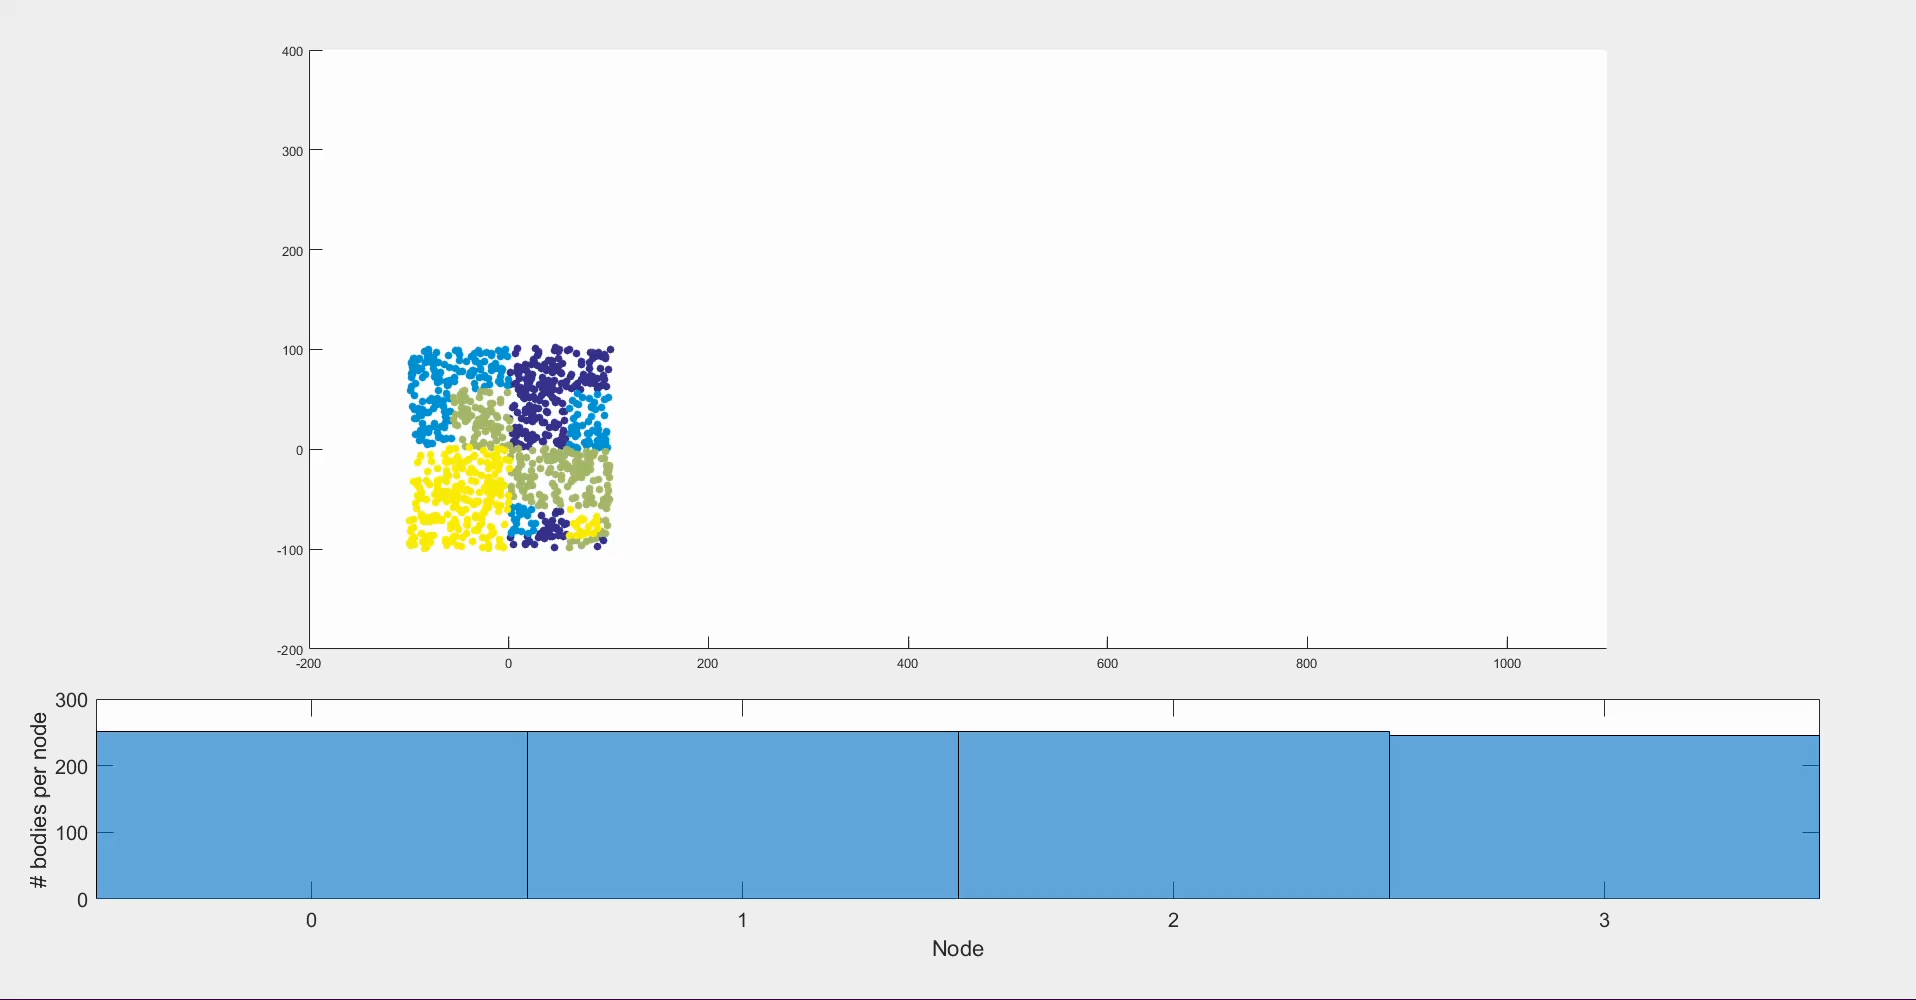
\includegraphics[width=1.0\linewidth]{load-balancing-poster.png}}{load-balancing.mp4}
  \end{center}
\end{frame}

\begin{frame}
  \frametitle{Brute-force speed-up}
  \inputTikz{0.725}{../figures/speedup_bf.tex}
\end{frame}

\begin{frame}
\frametitle{Brute-Force speed-up}
\begin{itemize}
  \item For both sizes, Amdahl's law over estimated the real speedup
  \item Even for $10^5$ bodies, more than 32 nodes can still be interesting
  \item Irregular speedup curve possibly due to splitting of nodes between racks, hence significantly larger communicatoin times for some cases
\end{itemize}
\end{frame}

\begin{frame}
  \frametitle{Barnes-Hut (QT) speed-up}
  \inputTikz{0.725}{../figures/speedup_qt.tex}
\end{frame}

\begin{frame}
\frametitle{Barnes-Hut (QT) speed-up}
\begin{itemize}
  \item Amdahl predicts a very poor speedup... which is respected
  \item The problem comes from writing the data at each time step
  \item But significantly faster than brute-force approach
\end{itemize}
\end{frame}



